\documentclass{article}
\usepackage[left=1cm, right=1cm]{geometry}
\usepackage{amsmath}
\usepackage{multicol}
\usepackage{graphicx}
\usepackage{subcaption}
\usepackage{listings}
\usepackage[utf8]{inputenc}
\setlength{\columnsep}{1cm}

\lstdefinestyle{snipps}{
    basicstyle=\tiny,
    breakatwhitespace=false,
    breaklines=true,    
    tabsize=1,
    frame=single
}
 
\lstset{style=snipps}

\title{
    \textbf{Programação 3D} \\
    Relatório Técnico da Primeira Entrega \\
    Grupo 9
}
\author{Afonso Mercier (83416) \and Pedro Quintas (83546) \and Pedro Caldeira (81888)}
\date{}

\begin{document}
    \maketitle

    \begin{multicols}{2}
    \section{Funcionamento do Programa}

    O trabalho desenvolvido consiste numa aplicação de ray tracing na linguagem
    C++. O programa pode ser configurado para ler um ficheiro NFF e produz uma
    imagem fotorrealista com base na cena descrita no ficheiro.

    O desenvolvimento focou-se nos seguintes aspetos:

    \begin{itemize}
        \item Leitura de ficheiros NFF.
        \item Cálculo dos Raios Primários
        \item Cálculo da componente local da cor.
        \item Suporte para múltiplas fontes luminosas.
        \item Sombras de contorno rígido.
        \item Reflexão de raios.
        \item Refração de raios.
        \item Intersecções de raios com algumas primitivas.
    \end{itemize}

    \section{Leitura de Ficheiros NFF}
    
    A leitura dos ficheiros que definem a cena foi é realizado por um \textit{parser} implementado, usando um \textit{switch-case}. Este \textit{parser} lê todos os ficheiros válidos no formato \textit{nff}, não validando qualquer tipo de valores, nem a ordem pela qual os elementos da cena são especificados. Isto permite, portanto que sejam lidos alguns ficheiros que não são considerados como válidos.\par 
    Estes casos não foram considerados como um problema no âmbito da cadeira e, caso o ficheiro não seja válido, não é garantido o funcionamento correcto do programa.\par
    O \textit{parser} implementado lê cada linha do ficheiro separadamente, criando o elemento correspondente na cena. Caso seja necessário ler mais que uma linha do ficheiro para especificar completamente um objecto (e.g. \textit{poligon patch}), são lidas linhas extraordinárias de forma a obter a informação completa do objecto. Após lidas todas as linhas que especificam um objecto na cena, o objecto é criado.
    

    \section{Raios Primários}

    O algoritmo de \textit{Ray Tracing} começa com o lançamento de raios em direção aos pixeis da imagem.
    Estes raios são os raios primários e vão por sua vez criar mais raios de modo a calcular sombras, reflexões
    e refrações, os raios secundários.
    
    Para calcular os raios primários utilizamos a função \verb|calculatePrimaryRay| que recebe as coordenadas
    do ecrã do ponto para o qual quer lançar um raio e devolve o raio com origem na câmera e direção ao ponto.
    Para calcularmos a direção do raio é necessário passar das coordenadas do ecrã para o referencial do mundo.
    Para tal começarmos por passar o ponto para coordenadas da câmera e dado que o referencial da câmera em
    relação ao mundo é bem conhecido, passar para coordenadas do mundo é um problema trivial. O referencial
    da câmera é composto por 3 vetores que podem ser calculados a partir da direção da câmera,
    $\vec{at}$ e a normal ao chão, $\vec{up}$. O versor $\hat{z}$ do referêncial é paralelo a $\vec{at}$ e unitário;
    a direção versor $\hat{x}$ pode ser calculada através do produto externo $\hat{z} \times \vec{up}$ e é únitário;
    finalmente, $\hat{y} = \hat{z} \times \hat{x}$.
    
\begin{lstlisting}[language=C++]
Vector3 Camera::GetRefY() {
	return externalProduct(GetRefZ(), GetRefX());
}

Vector3 Camera::GetRefZ() {
	return vector3MultScalar(normalize(subVector(at, eye)), -1);
}

Vector3 Camera::GetRefX() {
	return normalize(externalProduct(up, GetRefZ()));
}
\end{lstlisting}
    
    É necessário ainda calcular as dimensões do plano de projeção no mundo. Isto é feito aplicando diretamente a
    formula da tangente.
    
\begin{lstlisting}
float Camera::GetPlaneHeight() {
	return 2 * nearC * tan(angle / 2);
}

float Camera::GetPlaneWidth() {
	return (GetResX() / GetResY()) * GetPlaneHeight();
}
\end{lstlisting}

    Finalmente, as coordenadas do ponto em coordenadas são calculadas calculando a posição do ponto relativamente
    ao centro do plano de projeção e o valor da terceira componente corresponde sempre à distância do plano de
    projeção à câmera.
    
\begin{lstlisting}
Ray calculatePrimaryRay(int x, int y, Camera* cam) {
    float df = cam->GetHither();
    float w = cam->GetPlaneWidth();
    float h = cam->GetPlaneHeight();
    
    Vector3 rx = cam->GetRefX();
    Vector3 ry = cam->GetRefY();
    Vector3 rz = cam->GetRefZ();
    
    float cx = w * ((x + 0.5) / cam->GetResX() - 0.5);
    float cy = h * ((y + 0.5) / cam->GetResY() - 0.5);
    float cz = -df;
    
    Vector3 vx = vector3MultScalar(rx, cx);
    Vector3 vy = vector3MultScalar(ry, cy);
    Vector3 vz = vector3MultScalar(rz, cz);
    
    Vector3 d = addVector(vx, addVector(vy, vz));
    
    Ray ray;
    ray.versor = normalize(d);
    ray.origin = cam->GetFrom();
    
    return ray;
}
\end{lstlisting}
    
    \section{Componente Local da Cor}

    Caso um raio não intersecte nenhum objeto da cena, a sua cor corresponde
    à cor de fundo. No entanto, assim que é detetada uma intersecção, a
    primeira coisa a fazer é calcular a componente local da cor. Isto é a cor
    que resulta diretamente da influência das luzes da cena sobre o material
    do objeto.

    Para isto utilizamos o modelo de iluminação de Blinn-Phong. Este consiste no
    cálculo das componentes difusa e especular da cor. A componente difusa depende
    da direção da luz e da normal no ponto e é dada por
    $ Cor_{difusa} = k_d (\vec{n} \cdot \vec{l}) \cdot Cor_{material} $.

\begin{lstlisting}[language=C++]
float diffuse_c = clamp(col.object->_matProps->diffuseComp * internalProduct(col.normal, lightDirection), 0, 1);
Color diffuse = colorTimesConstant(col.object->_matProps->color, diffuse_c);
color = addColors(color, diffuse);
\end{lstlisting}

    A componente especular depende da normal e do vetor \textit{halfway}, que fica a meio
    entre a direção do raio e a direção da fonte luminosa, e é dada por
    $ Cor_{especular} = k_e (\vec{n} \cdot \vec{h})^{shine} \cdot Cor_{luz} $.

\begin{lstlisting}[language=C++]
Vector3 halfway = normalize(addVector(lightDirection, vector3MultScalar(ray.versor, -1)));

if (col.object->_matProps->specularComp > 0) {
    float specular_c = col.object->_matProps->specularComp * pow(internalProduct(col.normal, halfway), col.object->_matProps->shine);
    Color specular = colorTimesConstant(light->color, specular_c);
    color = addColors(color, specular);
}
\end{lstlisting}

    \section{Fontes Luminosas}
    Para permitir a iluminação na cena por multiplas fontes de luz foi criada a estrutura  \verb|_positionallight|, a qual é instanciada para cada luz da cena. A cor de um determinado ponto é então calculada somando o valor de iluminação para cada fonte de luz.
\begin{lstlisting}[language=C++]
for (PositionalLight* light : scene->lights) {
    /* Verificar se a luz nao se encontra por tras do objecto*/
    /* calcular a compontente difusa e especular (caso necessario) e adicionar ao valor da cor*/
}
\end{lstlisting}
    \section{Sombras}

    Para calcular as sombras de contorno rígido, basta garantir que cada uma das fontes
    luminosas é efetivamente capaz de iluminar o ponto no qual estamos a calcular a
    iluminação. Para tal lançamos um raio auxiliar em direção à fonte luminosa, um
    \textit{shadow feeler}. Caso este raio intersecte algum objeto da cena antes de
    alcançar a fonte luminosa, esta fonte não tem impacto na cor final do ponto.

\begin{lstlisting}[language=C++]
Vector3 lightDirection = normalize(subVector(light->pos, col.point));
if (internalProduct(lightDirection, col.normal) <= 0) {
    // The Light is behind our object.
    continue;
}

Ray shadow_feeler;
shadow_feeler.versor = lightDirection;
shadow_feeler.origin = addVector(col.point, vector3MultScalar(lightDirection, EPSILON));
Collision shadow = scene->castRay(shadow_feeler);

// If the shadow feeler did not collide or if the collision was further away than the light source.
//Bling Phong model
if (shadow.object == nullptr || vector3Length(subVector(shadow_feeler.origin, shadow.point)) > vector3Length(subVector(light->pos, col.point))) {
    // Calculate the Blinn-Phong.
}
\end{lstlisting}

    É também de notar que caso o próprio objeto esteja a tapar a fonte luminosa, esta não
    tem impacto na cor final do objeto.

    \section{Reflexão}
    
    Quando um raio intersecta um objeto, caso a componente especular do material
    seja superior a zero, é necessário calcular a cor relativa à reflexão da
    cena no objeto. Este calculo é feito através de uma chamada recursiva à função
    \verb|rayTracing| utilizando um novo raio. O novo raio é calculado de modo
    a fazer um ângulo com a normal na colisão igual ao ângulo entre o raio incidente
    e a normal na colisão.

    A cor resultante desta reflexão é atenuada de acordo com a componente especular
    do material do objeto.

\begin{lstlisting}[language=C++]
if (col.object->_matProps->specularComp > 0 && depth < DEPTH_TRACE_LIMIT) {
    Ray reflector;
    reflector.versor = normalize(subVector(ray.versor, vector3MultScalar(col.normal, 2 * internalProduct(ray.versor, col.normal))));
    reflector.origin = addVector(col.point, vector3MultScalar(reflector.versor, EPSILON));

    Color reflected = colorTimesConstant(rayTracing(reflector, depth + 1, RefrIndex), col.object->_matProps->specularComp);
    color = addColors(color, reflected);
}
\end{lstlisting}

    O raio criado é ligeiramente deslocado, de modo a evitar intersecções com o objeto refletor. Dada a natureza recursiva do algoritmo de \textit{Ray Tracing} é necessário
    limitar a profundidade que o algoritmo pode alcançar.

    \section{Refração}

    Quando um raio intersecta um objeto translúcido a sua direção é alterada
    de acordo com a lei de Snell. Visto que um raio tem uma direção única, é criado
    um novo raio e a cor resultante deste raio é atenuada de acordo com
    a transmitância do objeto. A direção do novo raio é resultante da aplicação
    da lei de Snell, $\eta_1/\eta_2 = sin(\theta_1)/sin(\theta_2)$.

\begin{lstlisting}[language=C++]
if (col.object->_matProps->t > 0 && depth < DEPTH_TRACE_LIMIT) {
    Ray refractor;

    float origin_ior = RefrIndex;
    float dest_ior = col.inside ? 1.0f : col.object->_matProps->idxOfRefraction;
    Vector3 v = vector3MultScalar(ray.versor, -1);
    float ior = origin_ior / dest_ior;
    Vector3 vt = subVector(vector3MultScalar(col.normal, internalProduct(v, col.normal)), v);
    float sin_theta_t = ior * vector3Length(vt);
    float cos_theta_t = sqrt(1 - sin_theta_t * sin_theta_t);
    Vector3 t = normalize(vt);

    refractor.versor = normalize(addVector(vector3MultScalar(t, sin_theta_t), vector3MultScalar(col.normal, -cos_theta_t)));
    refractor.origin = addVector(col.point, vector3MultScalar(refractor.versor, EPSILON));

    Color refracted = colorTimesConstant(rayTracing(refractor, depth + 1, dest_ior), col.object->_matProps->t);
    color = addColors(color, refracted);
}
\end{lstlisting}

    Para aplicar a lei de Snell é necessário primeiro descobrir os índices de
    refração do meio em que o raio está a viajar e do novo meio em que o raio
    vai entrar. Convenientemente, a função \verb|rayTrace| tem como argumento
    o índice de refração do material em que o raio se está a propagar. O
    índice de refração do novo material pode ser ou o índice de refração
    do objeto que o raio intersectou, caso a colisão tenha acontecido fora
    do objeto, ou o índice de refração do ar, caso a colisão tenha acontecido
    dentro do objeto.

    Tal como com a reflexão, é necessário deslocar ligeiramente o raio refratado
    de modo a evitar intersecções com o próprio objeto.

    \section{Interseções}

    A cena a ser renderizada é composta por uma lista de primitivas geométricas,
    uma lista de cores e uma câmera. Para calcular a interseção de um raio com a cena,
    devemos calcular a interseção do raio com cada uma das primitivas existentes. Para este
    fim, fazemos uso do polimorfismo, criando uma classe \verb|Primitive| que representa
    qualquer primitiva geométrica, com uma função virtual \verb|intersect| que é concretizada
    em cada uma das primitivas concretas. A verdadeira interseção é aquela que tem um valor $t$
    menor, ou seja, a que ocorreu mais perto da câmera.

\begin{lstlisting}[language=C++]
Collision Scene::castRay(Ray ray) {
	Collision col;
	col.object = nullptr;
	for (Primitive* p : primitives) {
		Collision ncol = p->intersect(ray);
		if (col.object == nullptr || vector3Length(subVector(ncol.point, camera->GetFrom())) < vector3Length(subVector(col.point, camera->GetFrom()))) {
			col = ncol;
		}
	}
	return col;
}
\end{lstlisting}

    \subsection{Esferas}
    A interseção entre o raio e a esfera foi calculada  parametrizando a esfera e o raio, restringindo ambas as  equações para obter os pontos que satisfazem o sistema de equações e o respectivo $ t_{colisao}$. 
    Sendo importante de salientar a optmizição realizada ao testar se o valor calculado para b não é inferior a 0, uma vez que significaria que o raio aponta no sentido contrario ao centro da esfera, podendo ser descartada a interseção.   
    Para calcular o ponto de interseção é realizada a substituição do valor de $ t_{colisao}$ na equação do raio.
    A normal do ponto de interseção é calculada subtraindo o ponto da interseção à origem da esfera.

    \subsection{Planos Infinitos}
    Para calcular intersecções entre os raios e planos infinitos começamos por testar se o produto interno entre a normal do plano e o versor da direção do raio é igual a 0, se for, a interseção não é computada (sendo descartada) uma vez que significa que o plano e o raio são paralelos. De seguida, parametrizamos a equação do raio [$raio = o + t\vec{d} $] e do plano [$ (p_i - a) \cdot \vec{n} = 0$] para calcularmos o valor de  $ t_i$, onde ocorre a interseção, recorrendo à seguinte expressão:  $ t_i = -\frac{(o - a)\cdot \vec{n}}{\vec{n} \cdot \vec{d}}$. Caso $t_i < 0$ é descartado pois significa que a interseção ocorre atrás da origem do raio. Caso contrário o ponto é calculado substituindo $ t_i$ na expressão do raio, e a normal no ponto é a mesma que a do plano.
   
    
    \subsection{Triângulos}

    Para calcular a interseção entre um raio e um triângulo utilizamos o método de Möller-Trumbore,
    que consiste em resolver um sistema de três equações resultante da restrição da equação paramétrica do raio à equação implícita do plano definido pelo triângulo. Para além do parâmetro
    $t$, a resolução deste sistema resulta nas coordenadas baricêntricas do ponto da interseção. Os
    valores destas coordenadas podem depois ser usados para determinar se a interseção ocorreu no
    interior do triângulo. O sistema pode ser escrito na sua forma matricial.
    $$
        \begin{bmatrix}
            a & b & c \\
            e & f & g \\
            i & j & k \\
        \end{bmatrix}
        \begin{bmatrix}
            \beta \\ \gamma \\ t
        \end{bmatrix}
        =
        \begin{bmatrix}
            d \\ h \\ l
        \end{bmatrix}
    $$
    onde, dados $v_1$, $v_2$ e $v_3$, os pontos do triângulo, $o$ a origem do raio e $r$ a
    direção do raio
    \begin{align*}
        (a, e, i) &= v_2 - v_1 \\
        (b, f, i) &= v_3 - v_1 \\
        (c, g, k) &= -r \\
        (d, h, l) &= o - v_1 \\
    \end{align*}
    A solução do sistema é dada através do cálculo de determinantes.
    $$
        \beta =
        \begin{vmatrix}
            d & b & c \\
            h & f & g \\
            l & j & k \\
        \end{vmatrix}
        D^{-1},
        \gamma =
        \begin{vmatrix}
            a & d & c \\
            b & h & g \\
            c & l & k \\
        \end{vmatrix}
        D^{-1},
        t =
        \begin{vmatrix}
            a & b & d \\
            e & f & h \\
            i & j & l \\
        \end{vmatrix}
        D^{-1}
    $$
    $$    
        D =
        \begin{vmatrix}
            a & b & c \\
            e & f & g \\
            i & j & k \\
        \end{vmatrix}
    $$
    Para a interseção ser válida, $\beta >= 0$, $\gamma >= 0$, $\beta + \gamma <= 1$ e $t > 0$.

    \subsection{AABBs}

    Uma AABB, \textit{Axis Alligned Bounding Box}, trata-se de um paralelepípedo cujas arestas estão
    alinhadas com os eixos. Para calcular a interseção de um raio com uma AABB utilizamos o algoritmo de
    Kay-Kajiya. Se considerarmos que uma AABB em três dimensões é o resultado da interseção de 3 lajes
    infinitas, cada uma paralela a dois dos eixos, o algoritmo consiste em calcular o maior valor $t$
    correspondente à entrada do raio numa das três lajes, e o menor valor $t$ correspondente à saída do
    raio de uma das três lajes. Caso o maior $t_{entrada} < t_{saida}$ podemos concluir que o raio
    interseta a AABB.
    
    Caso a origem do raio seja exterior à AABB, o ponto da interseção pode ser calculado a partir da
    expressão paramétrica do raio, utilizando como parâmetro o $t_{entrada}$. Caso contrário,
    utilizamos o $t_{saida}$. A normal à interseção, caso esta exista, é paralela ao eixo perpendicular
    à laje intersetada e tem sinal oposto ao sinal da componente do versor do raio paralela a esse
    eixo.

    \end{multicols}

    \newpage
    \section{Imagens}

    \begin{figure}[h!]
        \centering
        \begin{subfigure}{.2\linewidth}
            \centering
            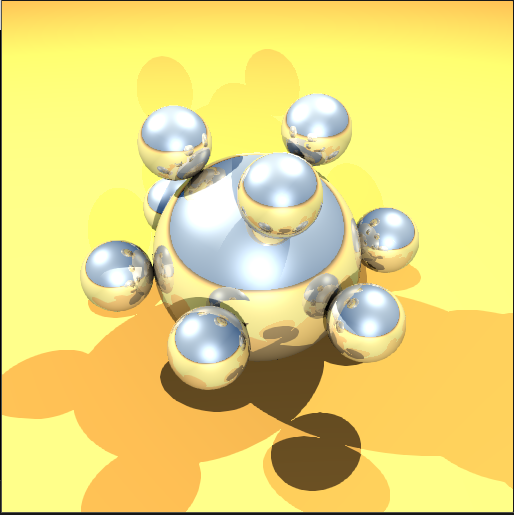
\includegraphics[width=\linewidth]{balls_low.png}
            \caption{balls\_low.nff}
            \label{fig:balls_low}
        \end{subfigure}
        \begin{subfigure}{.2\textwidth}
            \centering
            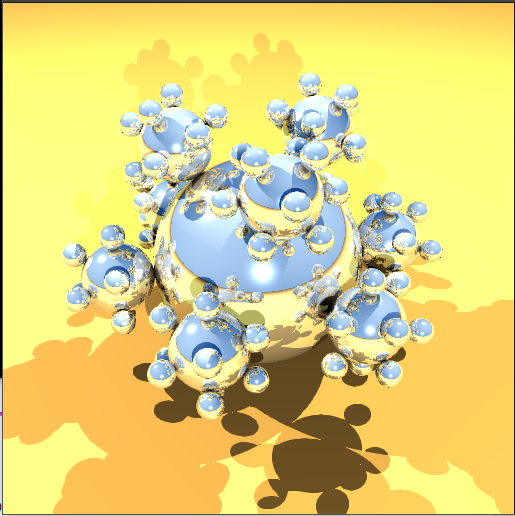
\includegraphics[width=\linewidth]{balls_medium.png}
            \caption{balls\_medium.nff}
            \label{fig:balls_medium}
        \end{subfigure}
        \begin{subfigure}{.2\linewidth}
            \centering
            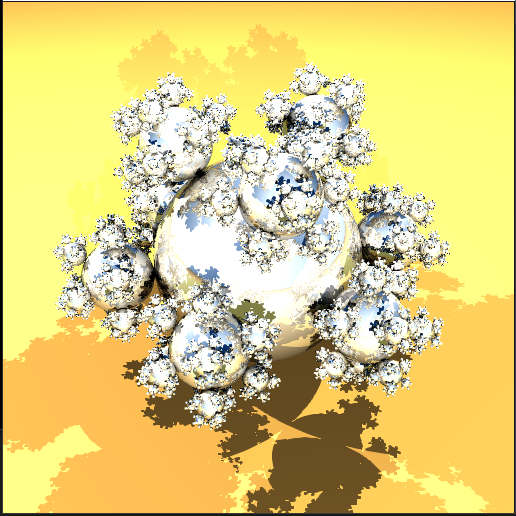
\includegraphics[width=\linewidth]{balls_high.png}
            \caption{balls\_high.nff}
            \label{fig:balls_high}
        \end{subfigure}

        \caption{Reflexões}
        \label{fig:balls}
    \end{figure}

    \begin{figure}[h!]
        \centering
        \begin{subfigure}[b]{.2\linewidth}
            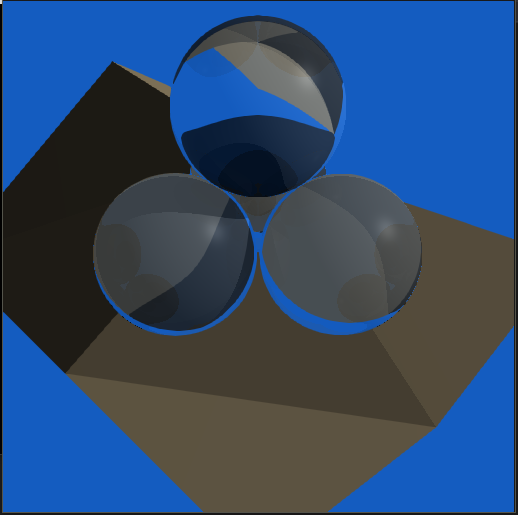
\includegraphics[width=\linewidth]{mount_low.png}
            \caption{mount\_low.nff}
            \label{fig:mount_low}
        \end{subfigure}
        \begin{subfigure}[b]{.2\linewidth}
            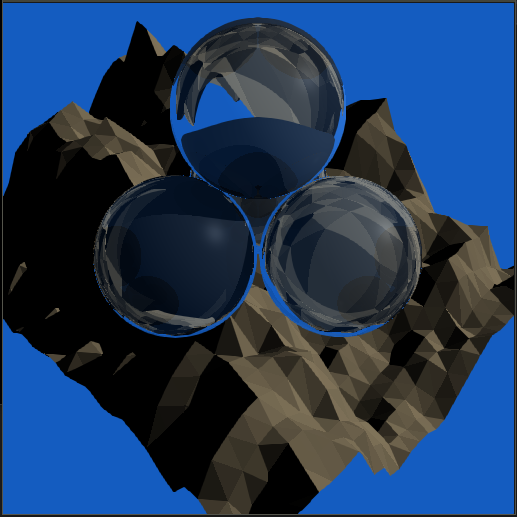
\includegraphics[width=\linewidth]{mount_high.png}
            \caption{mount\_high.nff}
            \label{fig:mount_high}
        \end{subfigure}
        \begin{subfigure}[b]{.2\linewidth}
            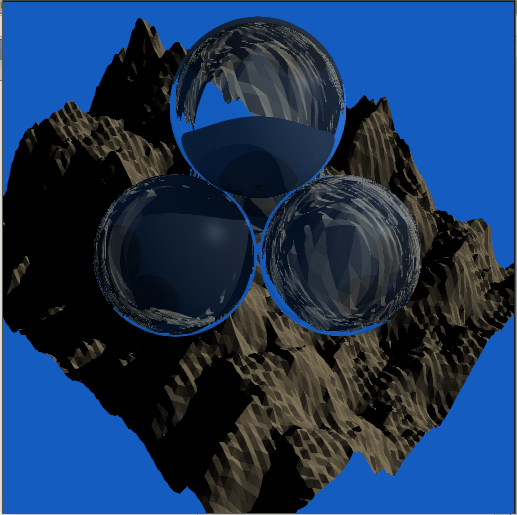
\includegraphics[width=\linewidth]{mount_very_high.png}
            \caption{mount\_very\_high.nff}
            \label{fig:mount_very_high}
        \end{subfigure}

        \caption{Refrações}
        \label{fig:balls}
    \end{figure}

    \begin{figure}[h!]
        \centering
        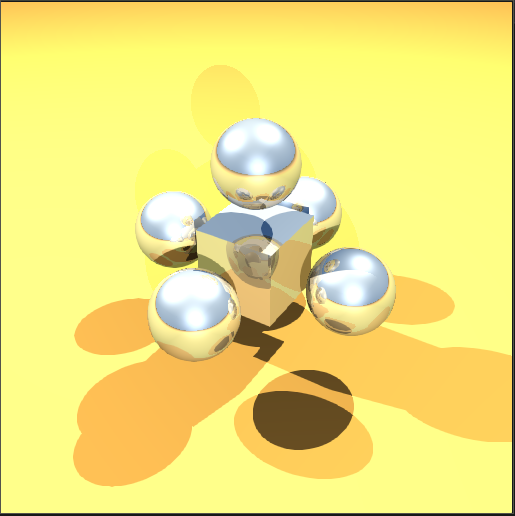
\includegraphics[width=.2\linewidth]{aabb.png}
        \caption{aabb.nff}
        \label{fig:aabb}
    \end{figure}

\end{document}